% Document class and two-column conversion
\documentclass{report}
% dimensions of paper and relative text positioning
\usepackage[a4paper,top=2cm,bottom=2cm,left=2cm,right=2cm]{geometry}
% package for including URLs
\usepackage{url}
% Required for including images
\usepackage{graphicx}
\usepackage{float} % Required for specifying the exact location of a figure

% enable writing in greek
\usepackage[greek]{babel}
\usepackage[utf8]{inputenc}
\usepackage[LGR]{fontenc}

\setlength{\parindent}{0pt} % Removes all indentation from paragraphs

% Start of the document
\begin{document}

% Set the language to greek
\selectlanguage{greek}

% Title page
\title{\Huge \bfseries Τεχνικές Βελτιστοποίησης \\ Δεύτερο Παραδοτέο} %\Huge and \bfseries are used to make the title bigger and bold
\author{Παπαδάκης Κωνσταντίνος Φώτιος\vspace{0.5cm} \\  ΑΕΜ:10371} % \vspace{0.5cm} is used to add some vertical space between the author and the AEM
\date{\today}
% prints the title, author and date on a separate page
\maketitle

% Table of contents page
\tableofcontents

% General introduction
\chapter{Εισαγωγή}
\section{Γενικά}
Η συνάρτηση πάνω στην οποία θα δουλέψουμε είναι η εξής:
$$f(x) = x^5 e^{-x^2-y^2}$$
Χρησιμοποιώντας ένα απλό visualization script σε Matlab εξάγουμε την παρακάτω εικόνα:
\begin{figure}[H]
    \centering
    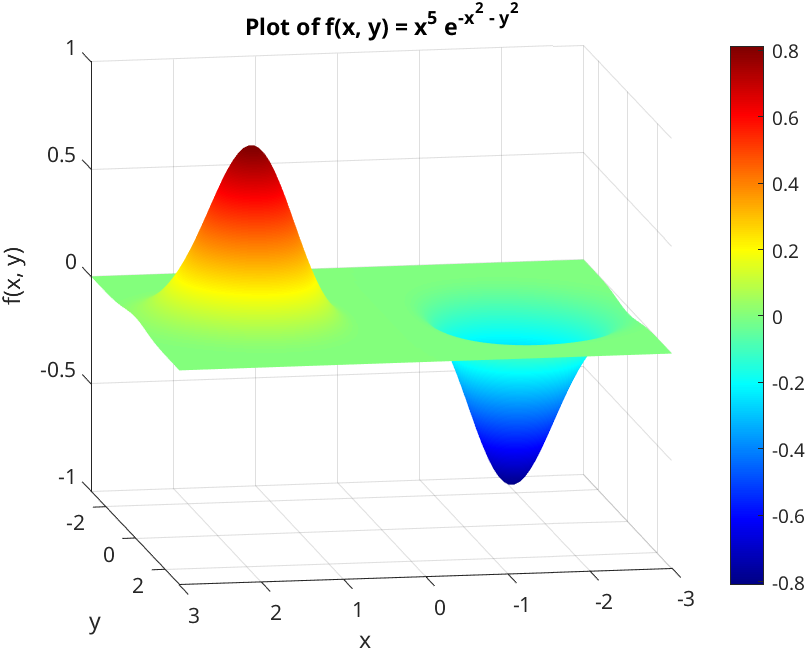
\includegraphics[width=0.5\textwidth]{media/visualization.png}
    \caption{Οπτικοποίηση της συνάρτησης $f(x,y)$}
\end{figure}
Ο τρόπος με τον οποίο εστιάσαμε σε αυτά τα χωρία $x$, $y$ είναι μέσω . 

Πρώτη Μερική Παράγωγος:
\begin{itemize}
    \item Ως προς το $x$:
    $$\frac{\partial{z}}{\partial{x}} = 5x^4e^{-x^2-y^2} - 2x^6e^{-x^2-y^2}$$
    $$\frac{\partial{z}}{\partial{x}} = x^4(5-2x^2)e^{-x^2-y^2}$$
    \item Ως προς το $y$:
    $$\frac{\partial{z}}{\partial{y}} = -2x^{5}ye^{-x^2-y^2}$$

\end{itemize}

Δεύτερη Μερική Παράγωγος:
\begin{itemize}
    \item Ως προς το $x$:
    $$\frac{\partial^2{z}}{\partial{x^2}} = 20x^{3}e^{-x^2-y^2}-22x^{5}e^{-x^2-y^2}+4x^{7}e^{-x^2-y^2}$$
    $$\frac{\partial^2{z}}{\partial{x^2}} = (20x^3 -22x^5 +4x^7)e^{-x^2-y^2}$$
    $$\frac{\partial^2{z}}{\partial{x^2}} = 2x^3(10-11x^2+2x^4)e^{-x^2-y^2}$$
    $$\frac{\partial^2{z}}{\partial{x^2}} = 2x^3(2x^2-1)(x^2-10)e^{-x^2-y^2}$$
    \item Ως προς το $y$:
    $$\frac{\partial^2{z}}{\partial{y^2}} = 4x^{5}y^{2}e^{-x^2-y^2} - 2x^{5}e^{-x^2-y^2}$$
    $$\frac{\partial^2{z}}{\partial{y^2}} = 2x^{5}(2y^2-1)e^{-x^2-y^2}$$
\end{itemize}

% Visualization of the function
\chapter{Θέμα 1}
\section{Εκφώνηση}
Σχεδιάστε την $f$ για να πάρετε μια γενική εικόνα της μορφής της.
\section{Λύση}



%  
\chapter{Θέμα 2}
\section{Εκφώνηση}

\section{Λύση}


% 
\chapter{Θέμα 3}
\section{Εκφώνηση}

\section{Λύση}


% 
\chapter{Θέμα 4}
\section{Εκφώνηση}

\section{Λύση}


% Comparison
\chapter{Ανάλυση Αποτελεσμάτων}
\section{Σύγκριση Μεθόδων}

\section{Σχόλια}


% Bibliography
\nocite{*} % Include all references in the bibliography, even if they are not cited in the report
\bibliographystyle{plain}
\bibliography{references/references} % We have to include the references somewhere in the report for them to show here if we don't use (\nocite{*})
\addcontentsline{toc}{chapter}{\bibname} % Add the bibliography to the table of contents

% End of the document
\end{document}